\documentclass[a4paper, 11pt]{article}

\usepackage[utf8]{inputenc}
\usepackage[english]{babel}

\usepackage{hyperref}

\usepackage{graphicx}
\usepackage{float}

\usepackage{listings}
\usepackage{xcolor}
\definecolor{listinggray}{gray}{0.9}
\definecolor{lbcolor}{rgb}{0.9,0.9,0.9}
\lstset{
	backgroundcolor=\color{lbcolor},
	tabsize=4,    
	language=[GNU]C++,
	basicstyle=\scriptsize,
	upquote=true,
	aboveskip={1.5\baselineskip},
	columns=fixed,
	showstringspaces=false,
	extendedchars=false,
	breaklines=true,
	prebreak = \raisebox{0ex}[0ex][0ex]{\ensuremath{\hookleftarrow}},
	frame=single,
	numbers=left,
	showtabs=false,
	showspaces=false,
	showstringspaces=false,
	identifierstyle=\ttfamily,
	keywordstyle=\color[rgb]{0,0,1},
	commentstyle=\color[rgb]{0.026,0.112,0.095},
	stringstyle=\color[rgb]{0.627,0.126,0.941},
	numberstyle=\color[rgb]{0.205, 0.142, 0.73},
}

\lstset{
	backgroundcolor=\color{lbcolor},
	tabsize=4,
	language=C++,
	captionpos=b,
	tabsize=3,
	frame=lines,
	numbers=left,
	numberstyle=\tiny,
	numbersep=5pt,
	breaklines=true,
	showstringspaces=false,
	basicstyle=\footnotesize,
	%  identifierstyle=\color{magenta},
	keywordstyle=\color[rgb]{0,0,1},
	commentstyle=\color{Darkgreen},
	stringstyle=\color{red}
}

\usepackage{fullpage}

\begin{document}
	\begin{centering}
		\large\textbf{Progress Report: 16/02/2017}\\
		~\\
		Oussama ENNAFII:
		\normalsize MATIS | TITANE \\
		Directors: Cl\'ement Mallet \& Florent Lafarge \\
	\end{centering}


	\section*{Data:}
	
	\begin{itemize}
		\item TODO:
			\begin{itemize}
				\item[-] I need to adapt my script for other XML formats and for tar file handling,

			\end{itemize}
		\item Misc:
			\begin{itemize}
				\item[-] Corrected Bati3D: February, 9th 2017, appointement with Yannick Couturier (DPR): to correct models they subdivid building footprints.
				\item[-] There is a new project producing hand annotated 3D models.
			\end{itemize}
	\end{itemize}
	
	\section*{Implementation:}
	Implementation status:
	\begin{itemize}
		\item Implemented:
			\begin{itemize}
				\item[-] Reader: 3DS and OFF,
				\item[-] Geomview viewer;
				\item[-] Automated testing;
				\item[-] Algorithms on bricks: area, contour length, affine transformations;
				\item[-] Project 3D models in 2D;
				\item[-] Occlusion management.
			\end{itemize}
		\item To add:
			\begin{itemize}
				\item[-] Project 3D model on Camera;
				\item[-] Save projections into georeferenced vectorial images using GDAL;
				\item[-] Rasterize projections for DSM comparison.
			\end{itemize}
		\item To complete:
			\begin{itemize}
				\item[-] Stitch Meshes (in order to stitch rooftops to facets);
				\item[-] Improve logging.
			\end{itemize}
	\end{itemize}
	
	\begin{figure}[H]
		\caption{\label{diag::class} Class diagram.}
		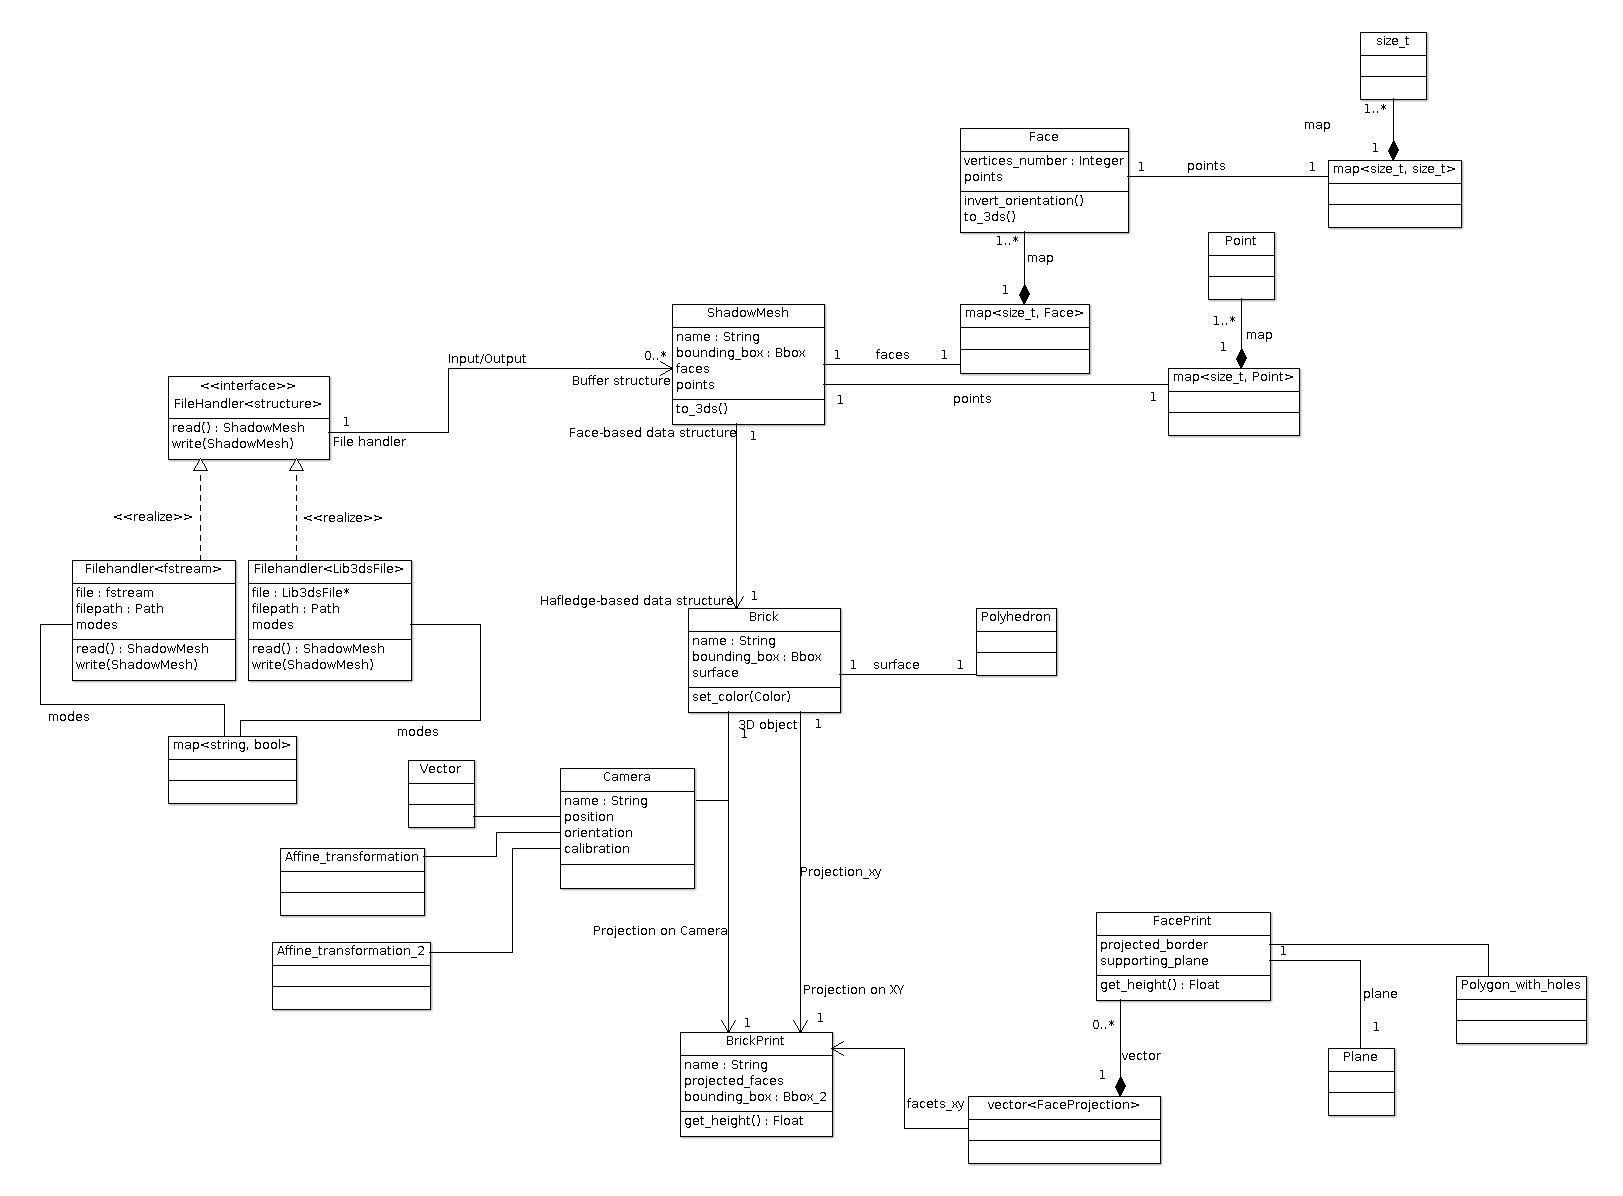
\includegraphics[scale=.3]{images/vectorial/class_diagram.png}
	\end{figure}
	
	\section*{Ideas:}
	There is nothing to report from the last time.
	
	\section*{Results:}
	There is no results to report for now.
	
	\section*{Attachments:}
	
	\begin{itemize}
		\item[-] You can checkout the Code in \href{https://github.com/Ethiy/3DSceneModel}{Github}.
	\end{itemize}
	
\end{document}
